% !TEX program = lualatex
        
% IMPORTANT! In order for the document to compile, one needs to use XeLaTeX or LuaLaTeX as compiler. This can be done in  Overleaf by Menu -> Settings -> Compiler -> Choose XeLaTeX/LuaLaTeX
\documentclass[t,24pt,aspectratio=169]{beamer}

\usepackage{UAM}
\usepackage{multicol} % Package for multiple coloumns
\usepackage[style=authoryear]{biblatex}
\usepackage{listings}
\usepackage{xcolor}

\definecolor{codegreen}{rgb}{0,0.6,0}
\definecolor{codegray}{rgb}{0.5,0.5,0.5}
\definecolor{codepurple}{rgb}{0.58,0,0.82}
\definecolor{backcolour}{rgb}{0.95,0.95,0.92}

\lstset{
	backgroundcolor=\color{backcolour},
	commentstyle=\color{codegreen},
	keywordstyle=\color{magenta},
	numberstyle=\tiny\color{codegray},
	stringstyle=\color{codepurple},
	basicstyle=\ttfamily\footnotesize,
	breaklines=true,
	frame=single,
	showstringspaces=false
}

%\usepackage{minted}
% lualatex -shell-escape -synctex=1 -interaction=nonstopmode archivo.tex

% \toplinje{Text at top} % The text at top. Remove the command if no text is desired


\addbibresource{references.bib}
\begin{document}

% The first slide. One can for instance change the main title, the subtitle, speaker, KU-unit, date and backgroundimage
{
\setbeamertemplate{background}{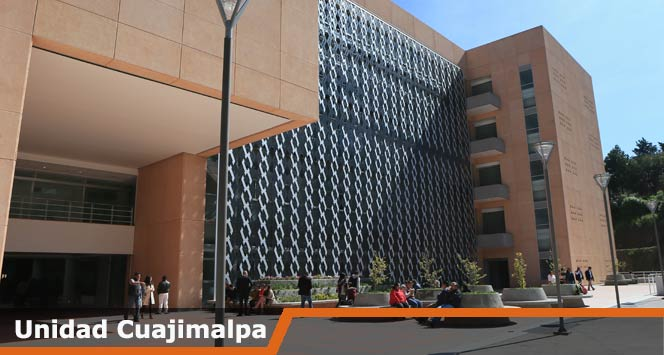
\includegraphics[width=\paperwidth,height=\paperheight]{uam/cua_05.jpg}}
\begin{frame}
    \begin{textblock*}{\textwidth}(0.53\textwidth,0.1\textheight)
        \begin{beamercolorbox}[wd=8.5cm,ht=7.3cm,sep=0.5cm]{hvidbox}
            \fontsize{5}{10}\fontfamily{ptm}\selectfont \textls[200]{UNIVERSIDAD AUTÓNOMA METROPOLITANA}
            \noindent\textcolor{KUrod}{\rule{6.8cm}{0.4pt}}
        \end{beamercolorbox}
    \end{textblock*}
    \begin{textblock*}{\textwidth}(0.53\textwidth,0.1\textheight)
        \begin{beamercolorbox}[wd=8.5cm,sep=0.5cm]{hvidbox}
                \Huge \textcolor{KUrod}{Integración de sistemas}
                \vspace{0.5cm}
                \par
                \Large Pila clásica de servicios web SOAP

                \vspace{0.5cm}
                \par
                \normalsize Juan Alvarado
        \end{beamercolorbox}
    \end{textblock*}
    \begin{textblock}{1}(14.5,11.38)
        % \includegraphics[width=1cm]{KU/KU-logo.png}
    \end{textblock}
\end{frame}
}


        %%%%%%%%%%%%%%%%%%%%%%%%%%%%%%%%%%%%%%%
	\begin{frame}[fragile, hvid]
		\frametitle{SOAP y XML como base de mensajería}
			\vfill
			\centering
			\Huge{SOAP y XML como base de mensajería}
			\vfill
	\end{frame}
%%%%%%%%%%%%%%%%%%%%%%%%%%%%%%%%%%%%%%%


%%%%%%%%%%%%%%%%%%%%%%%%%%%%%%%%%%%%%%%
	\begin{frame}[fragile, hvid]
		\frametitle{SOAP y XML como base de mensajería}
			\vfill
SOAP es un protocolo de mensajería para servicios web que encapsula datos en mensajes XML estructurados y transportados típicamente sobre HTTP o HTTPS.
\\~\\
			\vfill
	\end{frame}
%%%%%%%%%%%%%%%%%%%%%%%%%%%%%%%%%%%%%%%


%%%%%%%%%%%%%%%%%%%%%%%%%%%%%%%%%%%%%%%
	\begin{frame}[fragile, hvid]
		\frametitle{SOAP y XML como base de mensajería}
			\vfill
\begin{multicols}{2} 

Cada mensaje SOAP sigue una estructura estándar, lo que facilita la interoperabilidad entre plataformas distintas como Java, .NET o sistemas legados.
\\~\\
XML actúa como formato de representación, permitiendo describir datos complejos con tipos y estructuras anidadas.
\\~\\
\columnbreak
\centering
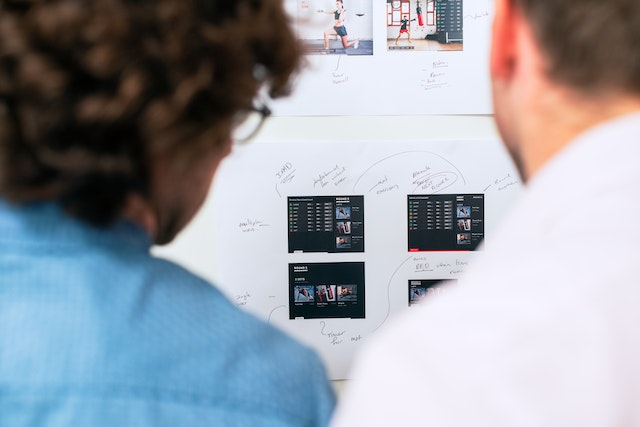
\includegraphics[width=6.6cm,height=5.9cm,keepaspectratio]{img/pexels-thisisengineering-3912478.jpg}
\end{multicols}
			\vfill
	\end{frame}
%%%%%%%%%%%%%%%%%%%%%%%%%%%%%%%%%%%%%%%


%%%%%%%%%%%%%%%%%%%%%%%%%%%%%%%%%%%%%%%
	\begin{frame}[fragile, hvid]
		\frametitle{SOAP y XML como base de mensajería}
			\vfill
Más adelante veremos con detalle la estructura de mensajes SOAP y de XML; aquí lo usamos como contexto para entender la pila de servicios web.
\\~\\
			\vfill
	\end{frame}
%%%%%%%%%%%%%%%%%%%%%%%%%%%%%%%%%%%%%%%


%%%%%%%%%%%%%%%%%%%%%%%%%%%%%%%%%%%%%%%
	\begin{frame}[fragile, hvid]
		\frametitle{WSDL: contratos estrictos}
			\vfill
			\centering
			\Huge{WSDL: contratos estrictos}
			\vfill
	\end{frame}
%%%%%%%%%%%%%%%%%%%%%%%%%%%%%%%%%%%%%%%


%%%%%%%%%%%%%%%%%%%%%%%%%%%%%%%%%%%%%%%
	\begin{frame}[fragile, hvid]
		\frametitle{WSDL: contratos estrictos}
			\vfill
\begin{multicols}{2} 

WSDL es un lenguaje basado en XML que describe qué operaciones ofrece un servicio, qué mensajes acepta y devuelve, qué tipos de datos utiliza y en qué endpoints están disponibles.
\\~\\
\columnbreak
\centering

\includegraphics[width=6.6cm,height=5.9cm,keepaspectratio]{img/young_man_wondering.jpg}
\end{multicols}
			\vfill
	\end{frame}
%%%%%%%%%%%%%%%%%%%%%%%%%%%%%%%%%%%%%%%


%%%%%%%%%%%%%%%%%%%%%%%%%%%%%%%%%%%%%%%
	\begin{frame}[fragile, hvid]
		\frametitle{WSDL: contratos estrictos}
			\vfill
En la práctica, WSDL funciona como un contrato estricto: herramientas pueden generar código cliente y servidor a partir del documento WSDL, y los mensajes se validan contra los esquemas definidos.
\\~\\
			\vfill
	\end{frame}
%%%%%%%%%%%%%%%%%%%%%%%%%%%%%%%%%%%%%%%


%%%%%%%%%%%%%%%%%%%%%%%%%%%%%%%%%%%%%%%
	\begin{frame}[fragile, hvid]
		\frametitle{WSDL: contratos estrictos}
			\vfill
Esta aproximación “contract-first” hace que cualquier desviación en el formato o tipo de dato cause errores claros, lo que da seguridad pero exige disciplina en la evolución del servicio.
\\~\\
			\vfill
	\end{frame}
%%%%%%%%%%%%%%%%%%%%%%%%%%%%%%%%%%%%%%%


%%%%%%%%%%%%%%%%%%%%%%%%%%%%%%%%%%%%%%%
	\begin{frame}[fragile, hvid]
		\frametitle{UDDI y la familia WS-}
			\vfill
			\centering
			\Huge{UDDI y la familia WS-}
			\vfill
	\end{frame}
%%%%%%%%%%%%%%%%%%%%%%%%%%%%%%%%%%%%%%%


%%%%%%%%%%%%%%%%%%%%%%%%%%%%%%%%%%%%%%%
	\begin{frame}[fragile, hvid]
		\frametitle{UDDI y la familia WS-}
			\vfill
\begin{multicols}{2} 

UDDI (Universal Description, Discovery and Integration) es un estándar basado en XML que define un registro o directorio para publicar y descubrir servicios web y la información técnica necesaria para consumirlos.
\\~\\
\columnbreak
\centering

\includegraphics[width=6.6cm,height=5.9cm,keepaspectratio]{img/pexels-realtoughcandycom-11035396.jpg}
\end{multicols}
			\vfill
	\end{frame}
%%%%%%%%%%%%%%%%%%%%%%%%%%%%%%%%%%%%%%%


%%%%%%%%%%%%%%%%%%%%%%%%%%%%%%%%%%%%%%%
	\begin{frame}[fragile, hvid]
		\frametitle{UDDI y la familia WS-}
			\vfill
Aunque los registros UDDI públicos han perdido protagonismo, el concepto de catálogo de servicios sigue vivo en portales de APIs modernos.
\\~\\
			\vfill
	\end{frame}
%%%%%%%%%%%%%%%%%%%%%%%%%%%%%%%%%%%%%%%


%%%%%%%%%%%%%%%%%%%%%%%%%%%%%%%%%%%%%%%
	\begin{frame}[fragile, hvid]
		\frametitle{UDDI y la familia WS-}
			\vfill
Alrededor de SOAP surgió también la familia de especificaciones WS- para abordar seguridad, confiabilidad, transacciones distribuidas y otros aspectos avanzados.
\\~\\
			\vfill
	\end{frame}
%%%%%%%%%%%%%%%%%%%%%%%%%%%%%%%%%%%%%%%


%%%%%%%%%%%%%%%%%%%%%%%%%%%%%%%%%%%%%%%
	\begin{frame}[fragile, hvid]
		\frametitle{UDDI y la familia WS-}
			\vfill
\begin{multicols}{2} 

Algunas de las especificaciones WS- más comunes son:
\\~\\
- WS-Security
\\~\\
- WS-Policy / WS-SecurityPolicy
\\~\\
- WS-Trust
\\~\\
- WS-SecureConversation
\\~\\
- WS-Addressing
\\~\\
\columnbreak
\centering

\includegraphics[width=6.6cm,height=5.9cm,keepaspectratio]{img/pexels-thisisengineering-3912976.jpg}
\end{multicols}
			\vfill
	\end{frame}
%%%%%%%%%%%%%%%%%%%%%%%%%%%%%%%%%%%%%%%


%%%%%%%%%%%%%%%%%%%%%%%%%%%%%%%%%%%%%%%
	\begin{frame}[fragile, hvid]
		\frametitle{UDDI y la familia WS-}
			\vfill
\begin{multicols}{2} 

Estos estándares complementan a SOAP y WSDL para formar lo que se conoce como la pila clásica de servicios web en entornos empresariales.
\\~\\
\columnbreak
\centering

\includegraphics[width=6.6cm,height=5.9cm,keepaspectratio]{img/pexels-thisisengineering-3913025.jpg}
\end{multicols}
			\vfill
	\end{frame}
%%%%%%%%%%%%%%%%%%%%%%%%%%%%%%%%%%%%%%%


%%%%%%%%%%%%%%%%%%%%%%%%%%%%%%%%%%%%%%%
	\begin{frame}[fragile, hvid]
		\frametitle{Actividad: Diseñar un mini‑contrato verbal}
			\vfill
Hacer cuatro equipos y trabajar un servicio de "Consulta de saldo" bancario.
\\~\\
Escriban en una hoja o documento: nombre de la operación, parámetros de entrada, estructura simplificada de la salida y posibles códigos de error.
\\~\\
			\vfill
	\end{frame}
%%%%%%%%%%%%%%%%%%%%%%%%%%%%%%%%%%%%%%%


%%%%%%%%%%%%%%%%%%%%%%%%%%%%%%%%%%%%%%%
	\begin{frame}[fragile, hvid]
		\frametitle{Actividad: Diseñar un mini‑contrato verbal}
			\vfill
\begin{multicols}{2} 

Luego discutan qué tan rígido debería ser este "contrato" para que diferentes equipos puedan implementarlo sin malentendidos.
\\~\\
Se trata de anticipar el rol de WSDL como contrato formal pero sin clavarse todavía en su sintaxis.
\\~\\
\columnbreak
\centering

\includegraphics[width=6.6cm,height=5.9cm,keepaspectratio]{img/pexels-thisisengineering-3862634.jpg}
\end{multicols}
			\vfill
	\end{frame}
%%%%%%%%%%%%%%%%%%%%%%%%%%%%%%%%%%%%%%%


{
	\setbeamertemplate{background}{
\includegraphics[width=\paperwidth,height=\paperheight]{uam/cua_01.jpg}}
	\begin{frame}[billede]
		\begin{textblock*}{\textwidth}(0\textwidth,0.77\textheight)
			\begin{beamercolorbox}[wd=7.8cm,sep=0.3cm]{rodbox}
				{\huge ¡Gracias!}
			\end{beamercolorbox}
		\end{textblock*}
	\end{frame}
}

%%%%% THIS IS THE BLOCK OF REFERENCES 

% \begin{frame}[hvid, allowframebreaks]
	% \frametitle{Referencias}
	% \printbibliography
	
	% \end{frame}


%%%%%% END OF THE BLOCK OF REFERENCES

\end{document}
